As presented in \autoref{chap:putinar} a polynomial barrier certificate can be constructed using \gls{sos} optimization by using the MATLAB toolbox SOSTOOLS. This toolbox is a convex relaxation framework based on sum of squares decompositions of multivariate polynomials and semidefinite programming solvers \citep{bib:prajna_framework} (for acquisition, see \autoref{app:sostools}).
In this chapter barrier certificates are sought with SOSTOOLS by use of Putinar's Positivstellensatz, presented in \autoref{def:putinar}.


\section{SOSTOOLS Syntax}
\vspace{-2mm}
An \gls{sos} program is the environment in which the \gls{sos} requirements in \autoref{def:barrier_sos} are set up, and searching for the barrier certificate corresponds to solving the \gls{sos} program.
This section is a short introduction to the SOSTOOLS formulation of the parameters and variables necessary to set up the requirements for the barrier certificate, based on the SOSTOOLS user guide \citep{bib:sostools_manual}.  
An overview of necessary \gls{sos} functions from the toolbox is given in \autoref{tab:sostools_syntax}.

\begin{table}[H]
\begin{tabularx}{\textwidth}{p{6cm} X}
\rowcolor{HeaderBlue}
\textbf{Syntax} & \textbf{Explanation}\\
\texttt{pvar x1;}\newline
\texttt{prog = sosprogram(x1);} & Initialization of an \gls{sos} program \texttt{prog} in the state variable \texttt{x1}, which is declared as  type \texttt{pvar} (or identically as \texttt{syms}, if the MATLAB symbolic toolbox is available)\\
\rowcolor{textBlue} 
\texttt{Z = monomials(x1,deg);}\newline
\texttt{[prog,q] = sossosvar(prog,Z);} & Parametrize an \gls{sos} polynomial \texttt{q} in the \gls{sos} program \texttt{prog}. The degree of the \gls{sos} polynomial is defined by the monomial vector \texttt{Z} of degree \texttt{deg} (i.e. deg(\texttt{q}) $=$ \texttt{deg}$^2$)\\
\texttt{Z = monomials(x1,deg);}\newline
\texttt{[prog,B] = sospolyvar(prog,Z);} & Parametrize a polynomial \texttt{B} in the program \texttt{prog}. The degree of the  polynomial is defined by the monomial vector \texttt{Z} of degree \texttt{deg} (i.e. deg(\texttt{B}) $=$ \texttt{deg})\\
\rowcolor{textBlue}
%\texttt{prog = soseq(prog,B-q);} & Declare the equality constraint \texttt{B-q} $=0$ in the \gls{sos} program \texttt{prog}\\
\texttt{prog = sosineq(prog,B-q);} & Declare the inequality constraint \texttt{B-q} $\geq 0$ (or more exact: \texttt{B-q} $\in\Sigma[x_1]$) in the \gls{sos} program \texttt{prog}\\
%\rowcolor{textBlue}
\texttt{prog = sossolve(prog);} & Solve the \gls{sos} program \texttt{prog} i.e. find coefficients for all polynomials conforming with all constraints \\
\rowcolor{textBlue}
\texttt{getB = sosgetsol(prog,B)} & After solving, get the solution (with coefficients) for the polynomial \texttt{B}\\
\texttt{[Q,Z,f] = findsos(getB-getq);} &  Test that the solution found complies with the requirement that the inequality is in fact \gls{sos}
\end{tabularx}
\caption{SOSTOOLS functions necessary to search for a barrier function as given by \autoref{def:barrier_sos}.}
\label{tab:sostools_syntax}
\end{table}

\vspace{-1mm}
An \gls{sos} program is initialized with the command \texttt{sosprogram}, and polynomials and \gls{sos} polynomials can be declared in the program in the variables that are input to the program (see \autoref{tab:sostools_syntax}) with \texttt{sospolyvar} and \texttt{sossosvar}, respectively.
%
%where \texttt{degrees} is the degrees of variables desired in the monomial; \texttt{[2 4]} would in this case give that \verb|Z = [x1^2; x1^4]| while \texttt{degrees = 0:2} would result in \verb|Z = [1; x1; x1^2]|. Declaring an SOS polynomial is done similarly to declaring an SOS variable
%
When the necessary SOS variables and polynomials are defined, the inequalities in \autoref{def:barrier_sos} can be defined with the function \texttt{sosineq}, and when all constraints are set up, the program is (attempted to be) solved by calling \texttt{sossolve}. This will return an overview of the precision of the solution (if any was found) as a residual error norm, number of iterations and time elapsed for solving the problem. To get the solution (coefficients) found for any of the SOS variables or polynomials, call the function \texttt{sosgetsol}.



%If no solution could be found, the degree (and thereby complexity) of some SOS variables or polynomials may be increased through their monomials, which may yield a solution to the SOS problem.



\section{Defining a Polynomial Barrier Certificate in SOSTOOLS}\label{sec:app_sostools_barrier_search}
\vspace{-2mm}

Searching for a polynomial barrier certificate in SOSTOOLS require the definition of all of the variables and polynomials given by \autoref{def:barrier_sos} as follows:
\vspace{-2mm}
\renewcommand{\labelitemii}{$\circ$}
\renewcommand{\labelitemiii}{$\bullet$}
\begin{itemize}
	\itemsep-0.7mm
	\item \textbf{Initialize the Program}\\
	First declare the state space variables $x\in\mathbb{R}^n$ as \texttt{syms} or \texttt{pvar}, and initialize the SOS program with the system states by the function \texttt{sosprogram}.
	\item \textbf{Define the Vector Field}\\
	The open-loop state space system $f_{ol}(x)$ is defined, and a controller is found according to pole placement or another preferred method. Then write the closed-loop system equation $f_{cl}$ in terms of the symbolic state vector.
	\item \textbf{Set up the Constraints for the Polynomial Barrier Certificate}\\
	Declare a monomial vector $Z_B$ in $x$ (or part of $x$) of sufficiently large degree, and parametrize the polynomial $B(x)$ as a function of $Z_B$ with \texttt{sospolyvar}.  
	The problem of finding the coefficients for the barrier certificate is now for each region $\mathcal{X}$, $\mathcal{X}_u$ and $\mathcal{X}_0$ a matter of defining the following:
	\vspace*{-1mm}
	\begin{itemize}
		\item \textbf{Define the Polynomials $g_j(x)$}\\
		Define one or more polynomials $g_j$ that are positive in the region to be defined and negative outside. Each polynomial may be solely a function of the robot tool position (and velocity) for static boundaries, and also a function of the heart position (and velocity) for dynamic boundaries. 
		\item \textbf{Declare the SOS Variables $q_j(x)$}\\
		Declare monomial vectors $Z_{q_j}$ in $x$ of appropriate degree (preferably as small as possible to keep the complexity of the problem as low as possible), and parametrize the SOS polynomials (multipliers) $q_j$ with \texttt{sossosvar}.
		\item \textbf{Set up the Inequality}\\
		Cf. the nonnegativity of an \gls{sos} polynomial ($q_0$), each \texttt{sosineq} can be formulated as given by  \autoref{def:barrier_sos}. For \autoref{cer2_putinar} choose a small positive number $\bar{\epsilon}$. The inequality pertaining to a set may be defined in terms of several $g_j$s; if the set is defined by
		\begin{itemize}
			\item $g_1 \bigcap g_2 \bigcap ... \bigcap g_m$, then write $h - \sum q_jg_j\geq 0$
			\item $g_1 \bigcup g_2 \bigcup ... \bigcup g_m$, then write $h - q_1g_1\geq 0$, $h - q_2g_2\geq 0$ etc.
		\end{itemize} 
		Note that each expression in the inequalities in \autoref{def:barrier_sos} must have even degrees in the leading and trailing terms in order for the expressions to be \gls{sos}.
	\end{itemize}
	\item \textbf{Solve the SOS Program}\\
	With all inequalities defined in the program, SOSTOOLS is now ready to solve for the barrier certificate with \texttt{sossolve}, if any certificate exists for the given system $f_{cl}(x)$. If no solution is found, increasing the degree of the \gls{sos} variables $q_j$ or the polynomial $B(x)$ may yield a solution. Otherwise it can be concluded that safety cannot be guaranteed of the  system under scrutiny. 
\end{itemize}





%\textcolor{red}{Matter of defining degree of B and qs - how to decide?}
%In the following section an example is given on how to search for a barrier certificate with SOSTOOLS.


%\textcolor{red}{Og hvordan bruger I så det. Kør eksemplet videre, så det er klart hvordan (8.2e) oversættes til SOS program. Jeg synes I skal køre eksemplet hele vejen igennem og idregne det i SOSTOOLS. På denne måde overbeviser i læseren og, at I kan oversætte teorien til praktisk implementation - Og dette giver points! }



\section{Barrier Certificate Search for First Order 1D System}
This section presents a simple example of a barrier certificate search for a 1D first order state space system with $x_1\in\mathcal{X}\subset\mathbb{R}$ corresponding to the robot slide joint being the only degree of freedom (see \autoref{fig:safe:overview} for an overview of the slide movement). First the system is defined, and a controller is designed with pole placement.
\begin{lstlisting}[language=matlab]
% Define state-space system with x1 = robot position
tau = 0.11; % time constant for the robot slide
A = -1/tau;
B = 1/tau;
K = place(A,B,[-10*1/tau]);
\end{lstlisting}
Then the symbolic state variables are declared for the SOS program in SOSTOOLS with the command \texttt{pvar}, which corresponds to the command \texttt{syms} in the Matlab symbolic toolbox. Now the SOS program \texttt{prog} can be initialized using the function \texttt{sosprogram} which takes the state variable(s) as input. For a short introduction to SOSTOOLS and its syntax, see \autoref{app:sostools}.
\begin{lstlisting}[language=matlab]
% Declare state variables
pvar x1

% Initialize the sum of squares program
prog = sosprogram(x1);
\end{lstlisting}
%The reference for the robot position is generated as the 1D heart position, taking into account the system gain $\bar{N}$, and the closed-loop system equation is written as a function of the sybolic state. %\textcolor{red}{Something is wrong with the reference..?}
The vector field or derivative of the state can now be defined in terms on the symbolic state variable. This function is necessary for the SOS program when requiring that the Lie derivative of the barrier certificate must be negative on the set $\mathcal{X}$.
\begin{lstlisting}[language=matlab]
% Vector field dx/dt = fx (closed loop)
fx = (A-B*K)*x1;
\end{lstlisting}
For ease of defining a (1D) function $g$ that is positive on an interval [$p_1\,\,\, p_2$], a parabola function is used.
\begin{lstlisting}[language=matlab]
function [a,b,c] = parabola(p1,p2)
a = -1;
b = a*(p1^2-p2^2)/(p2-p1);
c = -a*p1^2-b*p1;
end
\end{lstlisting}
Now declare the polynomial barrier function with the command \texttt{sospolyvar}. To do this, a monomial vector must be specified with \texttt{monomials} (see the monomial example in \autoref{eq:monomial_example}), which takes as input the state variable(s) and the monomial degree(s). The monomial degrees for $B(x)$ are chosen as low as possible until a solution can be found. In this case a solution can be found for a degree of $B(x)$ that is 0:4.
\begin{lstlisting}[language=matlab]
% Declare polynomial barrier function
zB = monomials(x1,0:4);
[prog,Bx] = sospolyvar(prog,zB);
\end{lstlisting}
Now the region $\mathcal{X}$ can be defined for the slide region $\pm0.1$\,m using the Lie derivative inequality in \autoref{cer3_putinar}, which is defined with the command \texttt{sosineq}. The SOS polynomials $q$ are of the form in \autoref{eq:sos_polynomial} and are declared with the command \texttt{sossosvar}, also taking a monomial vector as input.
\begin{lstlisting}[language=matlab]
% Define space X in R^n
[a,b,c] = parabola(-0.1,0.1); % get coefficients for parabola which is positive for x in [-0.1,0.1]
gX = a*x1^2+b*x1+c;
zX = monomials(vars,0:2);
[prog,qX] = sossosvar(prog,zX);
prog = sosineq(prog,-diff(Bx,x1)*fx-gX*qX);
\end{lstlisting}
Similarly, the region $\mathcal{X}_u$ is defined according to the SOS inequality in \autoref{cer2_putinar} as the area between slide positions 5-10\,cm.
\begin{lstlisting}[language=matlab]
% Define space Xu in X
[a,b,c]=parabola(0.05,0.1);
gXu = a*x1^2+b*x1+c;
zXu = monomials(x1,0:2);
[prog,fXu] = sossosvar(prog,zXu);
prog = sosineq(prog,Bx-gXu*fXu);
\end{lstlisting}
And finally the region $\mathcal{X}_0$ is defined according to the SOS inequality in \autoref{cer1_putinar} as $\mathcal{X}\setminus\mathcal{X}_u$.
\begin{lstlisting}[language=matlab]
% Define space X0 in X
[a,b,c] = parabola(-0.1,0.05);
gX0 = a*x1^2+b*x1+c;
zX0 = monomials(x1,0:2);
[prog,fX0] = sossosvar(prog,zX0);
prog = sosineq(prog,-Bx-gX0*fX0);
\end{lstlisting}
With all three areas defined according to \autoref{eq:barrier_constraints_putinar}, the program is ready to be solved by using the command \texttt{sossolve}. If a solution is found, an overview of the solution accuracy is printed in the Matlab terminal as the residual norm, number of iteration steps and solving time. To get the polynomial $B(x)$ use the function \texttt{sosgetsol}.
\begin{lstlisting}[language=matlab]
% Solve for B
prog = sossolve(prog);
getB = sosgetsol(prog,Bx)
\end{lstlisting}
For this particular program, the solution barrier certificate is found to be
\begin{equation}
B(x) = 0.016168\cdot x_1^4 + 0.0064892\cdot x_1^3 + 0.00072547\cdot x_1^2 + 6.5473e\text{-}8\cdot x_1 - 2.7291e\text{-}6
\end{equation}
and is depicted in \autoref{fig:barrier_1storder_staticlim}.

\begin{figure}[htbp]
	\hspace*{-12mm}
	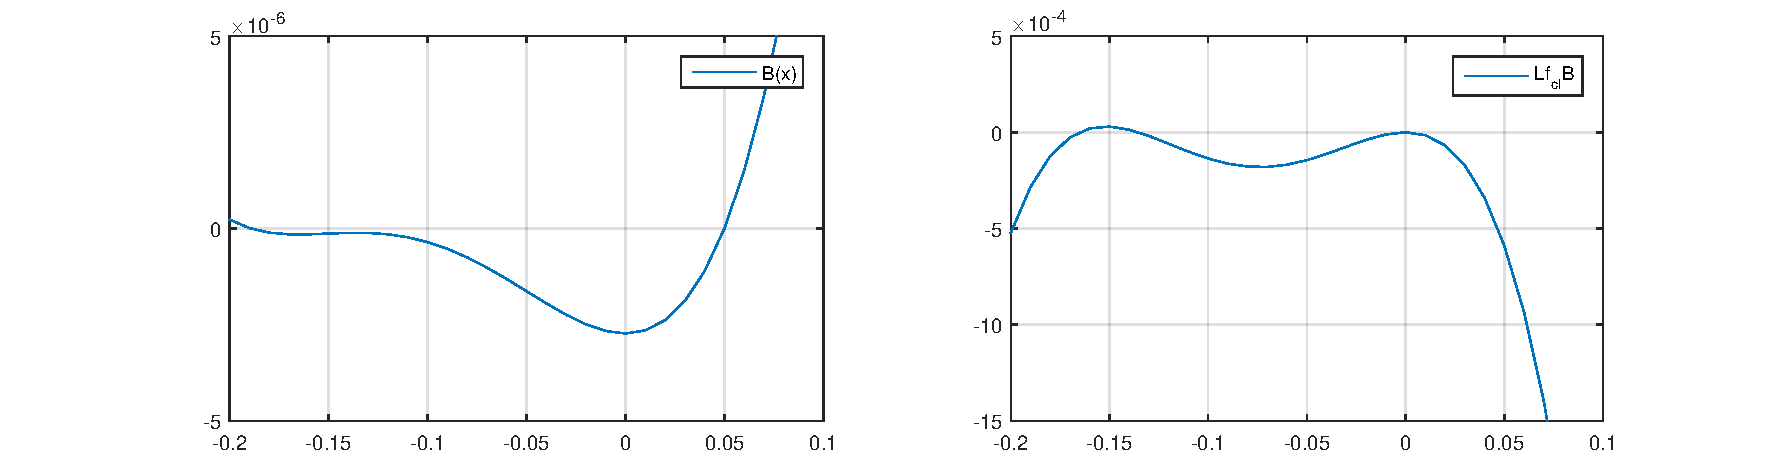
\includegraphics[width=1.1\textwidth]{1stordersys_staticlimits.pdf}
	\caption{A barrier certificate is found with SOSTOOLS that complies with the requirements in \autoref{eq:barrier_constraints}: it is positive on $\mathcal{X}_u=\{x_1\in [0.05,\,\,0.1]\}$ and negative on $\mathcal{X}_0=\{x_1\in [-0.1,\,\,0.05]\}$, and its Lie derivative is nonpositive on $\mathcal{X}=\{x_1\in [-0.1,\,\,0.1]\}$.}
	\label{fig:barrier_1storder_staticlim}
\end{figure}

or decreasing the region $\mathcal{X}_0$

\section{Safety Verification of First Order System}
First a linear open-loop state space system is defined according to the measurement of a step on the robot slide, showing a time constant $\tau=110$\,ms, giving the closed-loop system in \autoref{eq:1storder_1D_ss}:
\begin{equation}
\dot{x} = Ax+Bu = Ax+B(\bar{N}x_{ref}-Kx) = %-\tau^{-1}x+\tau^{-1}u=
-\tau^{-1}x+\tau^{-1}(\bar{N}x_{ref}-Kx)
\label{eq:1D_1storder}
\end{equation} 
which can be recast as the augmented state-space system
\begin{equation}
\dot{\tilde{x}}=
\dot{\begin{bmatrix}
	x_1\\x_{ref}
	\end{bmatrix}} =
\begin{bmatrix}
A-BK&B\bar{N}\\0&0
\end{bmatrix}
\begin{bmatrix}
x_1\\x_{ref}
\end{bmatrix}
= f_{cl}(x)
\label{eq:xtilde_1storder_1D}
\end{equation}
with no dynamics on the reference. A controller $K$ is found according to pole placement as described in \autoref{sec:K_Nbar_1D_1storder}, i.e. for the first order 1D system in \autoref{eq:1D_1storder} a controller that is 10 times faster than the system will be $K=9$. Similarly the system scaling factor $\bar{N}$ is determined according to the method described in \autoref{sec:K_Nbar_1D_1storder} as $\bar{N}=10$.
The independent state variables are defined and the SOS program initialized as described in \autoref{sec:app_sostools_barrier_search}.

%Now the $g_j$ functions in \autoref{eq:barrier_constraints_putinar} are constructed according to \autoref{fig:safe:overview}:
%\begin{itemize}
%%\itemsep-1.3mm
%\itemsep-0.7mm
%\item The set $\mathcal{X}$ is defined by constructing a (second order polynomial) function $g_{1}(x_1)\geq 0 \in [\Lambda_{\text{lim}-},\Lambda_{\text{lim}+}]= [-0.1,0.1]$\,m, delimiting the region of possible robot tool positions, and another function $g_2(x_{ref})\geq 0 \in [\Lambda_{h-}+\Delta,\Lambda_{h+}-\Delta]=[-0.1+\Delta,0.05-\Delta]$\,m, delimiting the region of allowable reference positions 
%\end{itemize}

The linear first order system from \autoref{eq:1storder_1D_ss} is defined with the same pole placement controller and thereby system gain as in \autoref{eq:K_1} and \ref{eq:barm_1}, and the same regions/intervals assigned for $\mathcal{X}$, $\mathcal{X}_u$ and $\mathcal{X}_0$ as given in \autoref{fig:safe:overview} - see \autoref{fig:intervals_for_sos}.
\begin{lstlisting}[language=matlab]
% 1D system WITH STATIC REFERENCE
clear all; clc; 

% Time constant from measurement
tau = 0.11;
% State-space matrices from first order open-loop system
A = -1/tau;
B = 1/tau;
% Setpoint controller that is xx times faster than the system
xx = 10;
K = place(A,B,[xx*A]);

C = 1;
D = 0;
Acl = A-B*K;
sysol = ss(A,B,C,D);
syscl = ss(Acl,B,C,D);

% Internal gain in the system for compensation of the reference
Nbar = -inv(C*inv(A-B*K)*B+D);

% Set upper and lower limits for the set intervals X, Xu and X0
Xmax = 0.1;
Xmin = -0.1;
Xumax = Xmax;
Xumin = 0.05;
X0max = Xumin;
X0min = Xmin;
\end{lstlisting}

\begin{figure}[htbp]
	\centering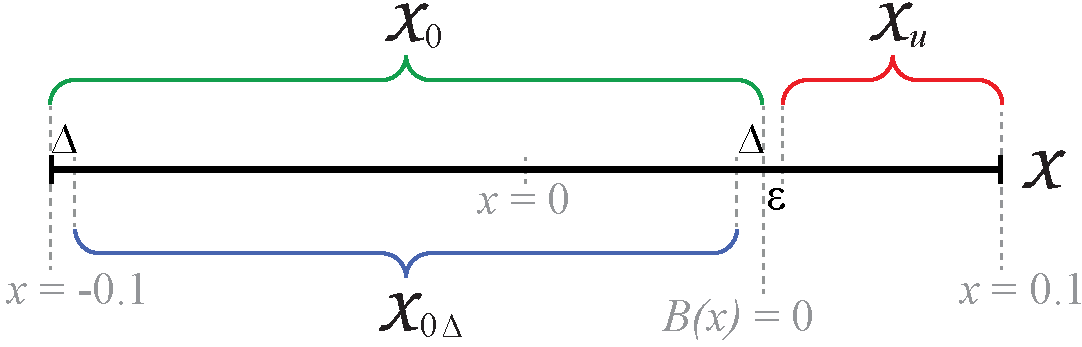
\includegraphics[width=0.6\textwidth]{intervals_for_sos.pdf}
	\caption{Intervals for the 1D case study, where the solid black line represents the interval $\mathcal{X}=\{x_1\in [-0.1, 0.1]\}$, and the interval $\mathcal{X}_0$ defines the interval where $B(x)\leq 0$, while $\mathcal{X}_u$ defines the interval where $B(x)>0$, separated from the zero level set by the small distance $\epsilon$. The interval $\mathcal{X}_{0\Delta} \subset \mathcal{X}_0$ is the interval of positions from which a reference can be taken $x_{ref}\in\mathcal{X}_{0\Delta}$. This interval is slightly smaller than the safe initial set $\mathcal{X}_0$, separated from the zero level set of $B(x)$ by the small distance $\Delta$.}
	\label{fig:intervals_for_sos}
\end{figure}

The small $\epsilon>0$ from \autoref{cer2_putinar} is defined "as small as possible", and another small $\Delta>0$ is introduced in order to be test for validity of a controller with references within the interval $\mathcal{X}_{0\Delta} \subset \mathcal{X}_0$ with a distance of at least $\Delta$ to the zero level set of $B(x)$, see \autoref{fig:intervals_for_sos}.
\begin{lstlisting}[language=matlab]
% Distance reference should keep to the unsafe region
delta = 0.001;

% Distance which the unsafe region is allowed to deviate from the desired zero level set specified by the g(x) defining Xu
epsilon = 0.00001;
\end{lstlisting}
The SOS program is initialized with the augmented state $\tilde{x}$ and thereby vector field as defined in \autoref{eq:xtilde_1storder_1D}. 
\begin{lstlisting}[language=matlab]
% =============================================
% Control Barrier Function Search for 1D system WITH STATIC REFERENCE
pvar x1 xref
xtilde = [x1; xref];

% =============================================
% First, initialize the sum of squares program
prog = sosprogram(xtilde);

% =============================================
% Vector field dt/dx = fx (closed loop)
fx = [A-B*K B*Nbar; 0 0]*xtilde;
\end{lstlisting}
The polynomial $B(x)$ is declared in as small degree "as possible". If any odd-order functions $g_j$ exist, $B(x)$'s leading term should be of an even degree higher than the uneven degree of the leading term of that $g_jq_j$. \textcolor{red}{It is considered that $B(x)$ should only be a function of the position and not of the reference, as the controller is considered as a static position setpoint controller for one single reference, and the program then tests the set of controllers, each with a setpoint within the interval $\mathcal{X}_{0\Delta} \subset \mathcal{X}_0$, for safety.}
\begin{lstlisting}[language=matlab]
% =============================================
% Declare polynomial degree of barrier function (FUNCTION OF BOTH X1 AND XREF?)
zB = monomials(x1,0:4);
[prog,Bar] = sospolyvar(prog,zB);
\end{lstlisting}
As $B(x)$ should be valid for the set $\mathcal{X}$, $\mathcal{X}$ is defined by $g_1(x_1)$ being positive on the slide interval, \textcolor{red}{and simultaneously $g_2(x_{ref})$ being positive on the interval $\mathcal{X}_{0\Delta} \subset \mathcal{X}_0$.} See \autoref{fig:intervals_for_sos} and \ref{fig:1D_static_gfunctions}.

\begin{figure}[htbp]
	\hspace*{-5mm}
	\subbottom[The $g(x_1)$ functions defining the sets $\mathcal{X}$, $\mathcal{X}_u$ and $\mathcal{X}_0$.]{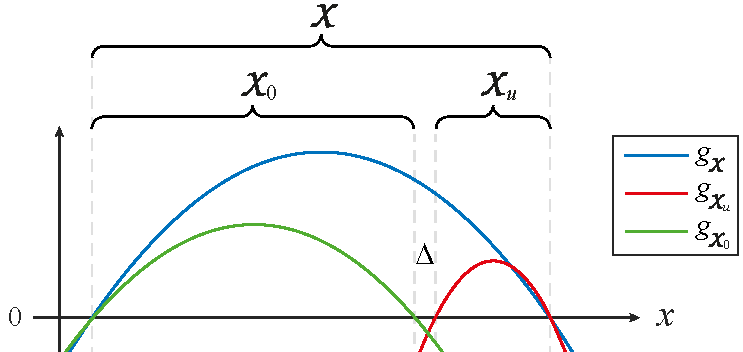
\includegraphics[width=0.55\textwidth]{1stordersys_staticlimits_g.pdf}\label{fig:1stordersys_staticlimits_g}}%
	\hspace{-2mm}
	\subbottom[The function $g(x_{ref})$ also used to define $\mathcal{X}$.]{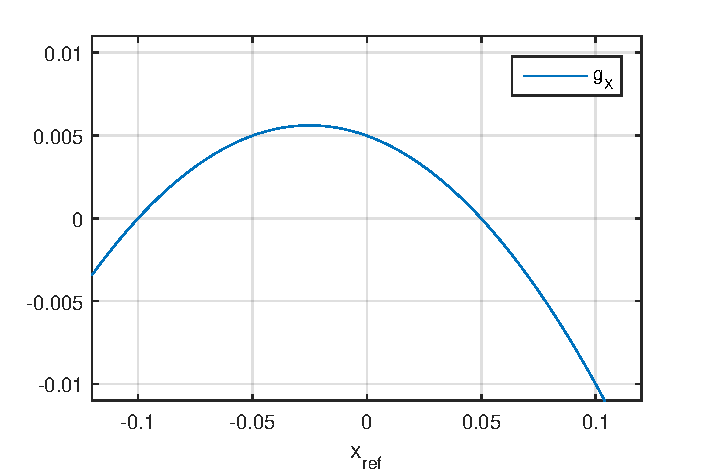
\includegraphics[width=0.55\textwidth]{1stordersys_staticlimits_gref.pdf}\label{fig:1stordersys_staticlimits_gref}}%
	\caption{The functions $g$ used to define the sets $\mathcal{X}$, $\mathcal{X}_u$ and $\mathcal{X}_0$ by the interval in which they are positive, i.e. $\mathcal{X}_u$ is defined by the interval where $g_{X_u}(x_1)$ is positive in \autoref{fig:1stordersys_staticlimits_g}. In the definition of the set $\mathcal{X}$, corresponding to the space where the barrier certificate is valid, also a function $g$ of the reference/setpoint is used. This means that the barrier certificate is valid for all controllers with setpoint within the interval where $g(x_{ref})$ is positive.}
	\label{fig:1D_static_gfunctions}
\end{figure}

\begin{lstlisting}[language=matlab]
% =============================================
% Define space X in Rn

% Define g1(x1) to be positive on the region that we want X to encompass
[a,b,c]=parabola(Xmin,Xmax); % get coefficients for parabola
gX1 = a*x1^2+b*x1+c;

% Declare SOS polynomials q1(xtilde) in the full state (CHOICE OF DEGREEE?)
zX1 = monomials(xtilde,0:2); 
[prog,qX1] = sossosvar(prog,zX1);

% With g2(xref) define X only on the interval of allowed references
[a,b,c]=parabola(X0min+delta,X0max-delta);
gX2 = a*xref^2+b*xref+c;

% Declare SOS polynomials q2(xtilde) (CHOICE OF DEGREE?)
zX2 = monomials(xtilde,0:2);
[prog,qX2] = sossosvar(prog,zX2);

% Setup SOS inequality according to Putinar's Positivstellensatz
prog = sosineq(prog,-[diff(Bar,x1) diff(Bar,xref)]*fx-gX1*qX1-gX2*qX2);
\end{lstlisting}
The unsafe set is defined as the interval where the position $x_1$ takes values between 5 and 10\,cm, see \autoref{fig:intervals_for_sos} and \ref{fig:1D_static_gfunctions}. \textcolor{red}{It is not clear whether also the reference should be part of the definition of $\mathcal{X}_u$ (with a $g_2(x_{ref})$ positive on the same interval as $g_1(x_1)$), it has been tested both with and without, but there is no clear indication from the results that is should or should not be included.}
\begin{lstlisting}[language=matlab]
% =============================================
% Define space Xu in X

% Define g1(x1) to be positive on the region that we want Xu to encompass
[a,b,c]=parabola(Xumin,Xumax);
gXu1 = a*x1^2+b*x1+c;

% Declare SOS polynomials q1(xtilde) in the full state (CHOICE OF DEGREEE?)
zXu1 = monomials(xtilde,0:3);
[prog,qXu1] = sossosvar(prog,zXu1);

% With g2(xref) define Xu outside the interval of allowed references
[a,b,c]=parabola(Xumin,Xumax);
gXu2 = a*xref^2+b*xref+c;

% Declare SOS polynomials q2(xtilde) (CHOICE OF DEGREE?)
zXu2 = monomials(xtilde,0:3);
[prog,qXu2] = sossosvar(prog,zXu2);

% Setup SOS inequality according to Putinar's Positivstellensatz
prog = sosineq(prog,Bar-epsilon-gXu1*qXu1);%-gXu2*qXu2);
\end{lstlisting}
\textcolor{red}{The same is the case for the definition of $\mathcal{X}_0$; it is defined as the safe position region, and it has been tested with and without the requirement of references in the interval $\mathcal{X}_{0\Delta} \subset \mathcal{X}_0$.}
\begin{lstlisting}[language=matlab]
% =============================================
% Define space X0 in X

% Define g1(x1) to be positive on the region that we want X0 to encompass
[a,b,c]=parabola(X0min,X0max);
gX01 = a*x1^2+b*x1+c;

% Declare SOS polynomials q1(xtilde) in the full state (CHOICE OF DEGREEE?)
zX01 = monomials(xtilde,0:4);
[prog,qX01] = sossosvar(prog,zX01);

% With g2(xref) define X0 only on the interval of allowed references
[a,b,c]=parabola(X0min+delta,X0max-delta);
gX02 = a*xref^2+b*xref+c;

% Declare SOS polynomials q2(xtilde) (CHOICE OF DEGREE?)
zX02 = monomials(xtilde,0:3);
[prog,qX02] = sossosvar(prog,zX02);

% Setup SOS inequality according to Putinar's Positivstellensatz
prog = sosineq(prog,-Bar-gX01*qX01);%-gX02*qX02);
\end{lstlisting}
In most cases the solution found has a leading term coefficient of order between -4 and -2, but very often the value of $B(x)$ is either positive or negative on the entire interval [-0.1,0.1]. \textcolor{red}{Strangely, in all tested combinations, $L_{f_{cl}}B(x)$ is positive-valued on an interval approximately [-0.02,0]. This and the fact that the zero level set of the barrier in no case is in $x=0.05$ makes it seem like we still haven't formulated the problem correctly in terms of the SOS description. We could use a little help to see what we do wrong.} 
\begin{lstlisting}[language=matlab]
% =============================================
% Solve for B
prog = sossolve(prog);
getB = sosgetsol(prog,Bar)

dBdx = [diff(getB,x1) diff(getB,xref)]

% =============================================
% Plot B and LfclB
figure
subplot(1,2,1);
Bx = plotB(getB,[Xmin,Xmax],0);
subplot(1,2,2);
LfclB = plotLfclB(dBdx,A,B,C,D,K,Nbar,[Xmin,Xmax]);
\end{lstlisting}

\textcolor{red}{It has been tried tweaking the constants $\epsilon$ and $\Delta$ as well as testing with all the monomial degrees $Z_B$, $Z_{X1}$, $Z_{X2}$, $Z_{u1}$, ($Z_{u2}$), $Z_{01}$, ($Z_{02}$), in degrees 0:2, 0:3, 0:4, and in/excluding the constraints from $x_{ref}$ on $\mathcal{X}_u$ an $\mathcal{X}_0$, but in no case $B(x)$ attains a shape that remotely reflects the requirements (on $x_1$) for $\mathcal{X}_u$ an $\mathcal{X}_0$.}
